\section{Qualitative Analysis - Quasi-Free Scattering $^{12}$C(p,2p)$^{11}$B}
Until the S444 experiment in 2020 CALIFA consisted out of a prototype frame filled with up to 64 CsI(Tl) crystals. The geometric coverage was therefore poor. For the S444 experiment CALIFA got its final frame and was fully filled in the forward barrel and 35\%filled in the iPhos region, CEPA was not installed yet. With these improvements it was possible to commission qfs-experiments with CALIFA at R3B. In the follow up experiment S467, also in 2020, the first experimental run to study single-particle structures of neutron-rich Ca isotopes via qfs-reactions was carried out.\newline
Even though great improvements in the detector development  were achieved the correction factors to correct for geometric acceptance would be much too high ( $\approx$ 10) for precise cross section measurements for qfs-reactions since the correction factors would in turn rely on a a simplified reaction model. A precise analysis of the acceptance correction factor and the development of a more sophisticated and data driven reaction model is out of the scope of this work. Therefore this analysis focusses on the methods of qfs-reaction identification and the extraction of the key informations dicussed in section \ref{sec:qfs_theo}. TODO: add more stuff here...\newline
\subsection{Setup-Calibration}
For setup description refer to section \ref{sec:analysis_cross_sec}. For all detectors except the SOFIA (Study On FIssion with Aladin) Time of Flight Wall the calibration parameters investigated by the respective detector-expert group were adopted. Herefore we will subsequently only describe the Time of Flight Wall calibration in this subsection.
\subsubsection{Flight-Path Reconstruction - SOFIA Time of Flight Wall}\label{subsec:flightpath_reco}
The procedure to calibrate the Time of Flight (ToF) Wall involves beforehand a precise flight-path reconstruction of the projectile from the entrance of Cave C downstream to the ToF Wall. Since only one tracking detector downstream to GLAD was in operation for the S444 experiment no angle of the deflected fragment/beam $\theta_{out}$ could be directly extracted. Herefore an advanced tracking algorithm was developed, motivated from ref. \cite{bertini2013study} (section 3.4). 
\begin{itemize}
\item The first step is to measure the scattering angle after target, $\theta_{in}$, and draw an extended line from the target position through the effective magnetic field of GLAD.  
\item Draw a trajectory line from the hit position in MWPC3 to the intersection point C (see figure \ref{fig:sub1_reco_path}) of the "kick-plane-line" and the reconstructed and extended track line upstream to GLAD.
\item Now sweep along the reconstructed track line upstream to GLAD. For each step a value for $\theta_{out}$ and $d1-d2$ is gathered, see figure \ref{fig:sub2_reco_path}.
\item As in figure \ref{fig:sub2_reco_path} shown, fit the data-points from previous step with a linear fit function and find the corresponding $\theta_{out}$ value where the fit line intersects with the abscissa. This corresponds to the case where $d1 = d2$. This is the approximated "kickpoint" in GLAD. 
\item Previous steps need to be executed for all events accordingly.
\end{itemize}
\begin{figure}[ht]
    \centering
    % First subfigure
    \begin{subfigure}[b]{0.70\textwidth}
        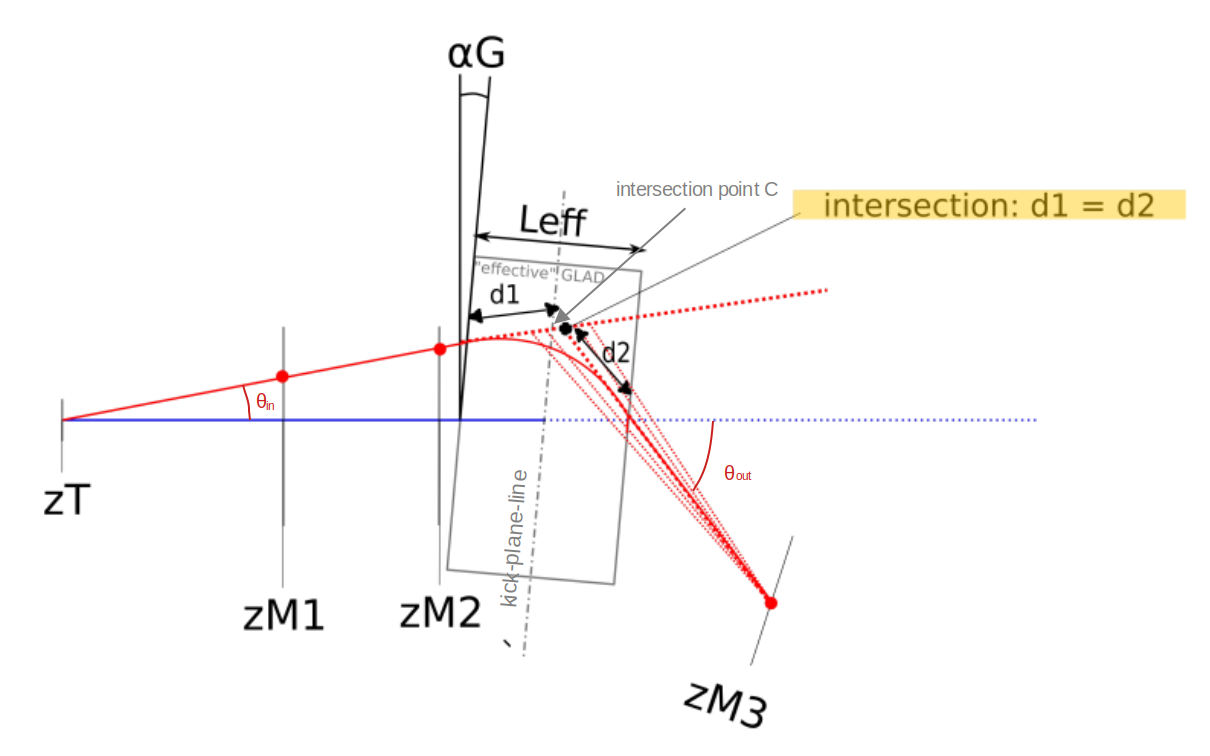
\includegraphics[width=\textwidth]{Figures/kick_point_algorithm.png}
        \caption{Flightpath reconstruction with "Leff" being the effective active width of the magnetic field of GLAD}
        \label{fig:sub1_reco_path}
    \end{subfigure}
    %\hfill % Optional: adds horizontal space between the figures
    % Second subfigure
    \begin{subfigure}[b]{0.25\textwidth}
        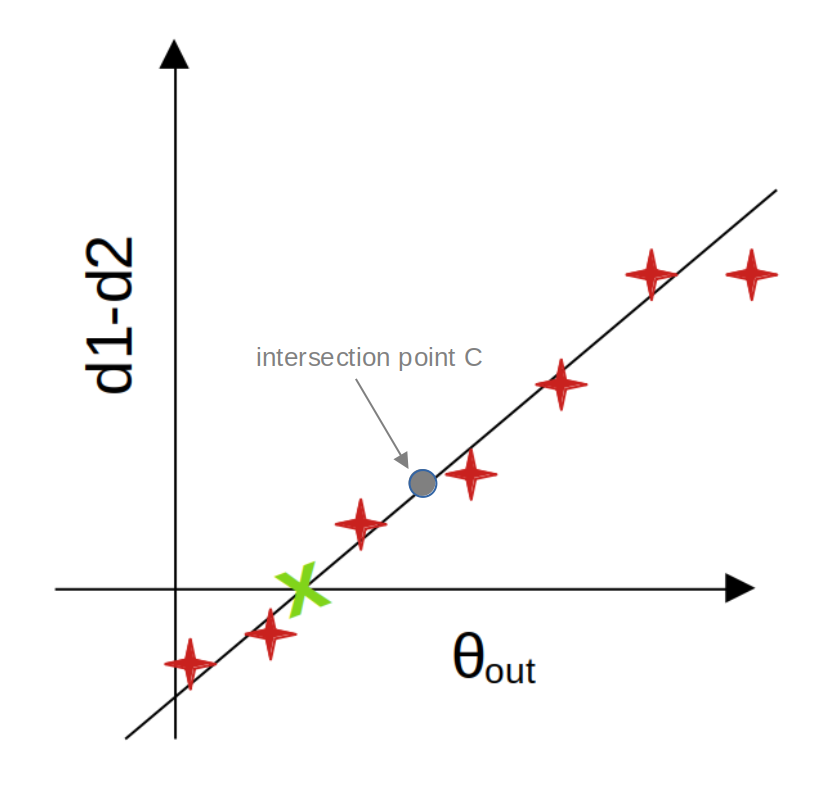
\includegraphics[width=\textwidth]{Figures/intersection_algorithm.png}
        \caption{$\theta_{out}$ approximation. For detailed information see text.}
        \label{fig:sub2_reco_path}
    \end{subfigure}

    \caption{Flightpath tracking and reconstruction of the fragment/beam after the target.}
    \label{fig:reco_path}
\end{figure}

Now that the scattering angle after the target $\theta_{in}$ and the angle after GLAD, $\theta_{out}$ is known and the position outside the magnetic field of GLAD are fixed, with $(z_1,x_1)$  the entrance point on the GLAD field and $(z_2,x_2)$ the exit point, the bending radius $r$ from the magnetic deflection can be determined:
\begin{equation}\label{eq:rho_glad}
r = \frac{L_{eff}}{2\,\cdot sin\left(\frac{\theta_{in}+\theta_{out}}{2}\right)\,\cdot cos\delta}
\end{equation}
where $L_{eff}$ is the effective active with of the magnetic field of GLAD, which correspons $\approx 2.06\,m$. This value could also be verified by extracting $L_{eff}$ from the formula for the magnetic rigidity $ B\cdot r = \gamma\beta \, m /q$ for empty target runs with known values of the B-field\footnote{For detector calibration, primarly for the ToFWall, we had several "empty sweep runs", with empty target and different B-field strenght settings. Those runs were optimal to validate $L_{eff}$.}.\newline
The angle $\delta$ in equation \ref{eq:rho_glad} is given by the trajectory line going through $(z_1,x_1)$/$(z_2,x_2)$ and the line parallel to the GLAD magnet width $L_{eff}$.\newline
A detailed derivation of equation \ref{eq:rho_glad} can be found in appendix \ref{app:flightpath}.
The arc trajectory $l_{GLAD}$ of the fragment within GLAD can be reconstructed using the bending radius $r$ and the entry and exit points $(z_1,x_1)$/$(z_2,x_2)$:
\begin{equation}\label{eq:arc}
l_{GLAD} = r \cdot \omega\qquad \text{with}\qquad \omega = 2\cdot asin(t_{1/2}{(2\cdot r)})
\end{equation}
where $\omega$ is the central angle and  $t_{1/2}$ is the cord length between $(z_1,x_1)$ and $(z_2,x_2)$.\newline
At this stage the full pathlength $L$ form the Start detector to the ToFW is fixed:
\begin{description}
\item \textbf{From Start to the target $l_{ST}$:} For this path section a straight flightpath parallel to the z-coordinate is assumed. The pathlength is taken from the position measurements of the Start detector and the target accordingly ($=118.3\,cm$). 
\item \textbf{Target to GLAD entrance point $(z_1,x_1)$, $l_{in}$:}For the  exact position assignment of $(z_1,x_1)$ both MWPC1 and MWPC2 position measurements have been calibrated with empty target runs by including an offset valuein order to center the x-position in both detectors around zero. From the position measurement of the central position of GLAD, its tilting angle $\alpha$ and $L_{eff}$ the intersection point of the fragment trajectory before GLAD and the "effective GLAD magnetic field rectangle", $(z_1,x_1)$, can be determined and with it the according flightpath section $l_{in}$.
\item \textbf{Arc trajectory within GLAD, ${l_{GLAD}}$:}This flightpath passage is determined by reconstructing $(z_1,x_1)$ and $(z_2,x_2)$, as it has been described in detail in the previous section. Hence the magnetic bending radius can be determined, see equation \ref{eq:rho_glad}, and finally the arc trajectory ${l_{GLAD}}$ as in equation \ref{eq:arc}.
\item \textbf{GLAD exit point $(z_2,x_2)$ to ToFW, $l_{out}$:}The hit position $(z_{MWPC3},x_{MWPC3})$ in MWPC3 is given by the reconstructed hit position in this detector and the position measurement of the detector itself. The exit point $(z_2,x_2)$ was reconstructed in the previous steps. Hence the trajectory line from $(z_2,x_2)$ to $(z_{MWPC3},x_{MWPC3})$ is fixed and is expanded to the intersection with the ToFW plane for the concluding $l_{out}$ measurement.  
\end{description}
The resulting flightpath $L$ recombines from:
\begin{align*}
L &= l_{ST}+l_{in}+l_{GLAD} + l_{out} 
\end{align*}
In the flightpath reconstruction the deflections in the y-dimension were omitted as the angular straggling in the target is small (TODO: give sigma value) and since the deflection of the fragment within GLAD is independent from its  y-position this contribution can be disregarded.


\subsubsection{Time of Flight Calibration -  SOFIA Start \& Time of Flight Wall}
For the time of flight measurement in the S444 setup the time is recorded and digitized by the VFTX,  VME-FPGA Time-to-Digital Converter (TDC) Modules based on tapped delay line (TDL) TDCs\cite{bayer2009development}. These modules provide for each detected signal a coarse time, is determined by counting cycles of a 200 MHz readout clock, resulting in a 5 ns binning resolution, and a fine time, which is obtained using an FPGA-based Time-to-Digital Converter (TDC), which employs a tapped delay line (TDL). In this approach, the signal propagates through a series of delayed logic modules within the FPGA until the subsequent clock cycle terminates the sampling process. The number of delay elements traversed by the signal is used to compute the time difference between the signal onset and the end of the clock cycle. The translation of the resulting fine time, with reasonable assumption of an uniform distribution, is achieved via a calibrated linear function. This procedure assigns to each preamplifier signal in the start detector (left/right) and the ToF Wall (up/down) a calibrated raw time \textit{raw\_t}:
\begin{align*}
raw\_t &= coarse\_time\_clocks  \cdot 5ns + offset[fine\_time]
\end{align*}
Finally, the raw time of flight is reconstructed by combinding all four time measurements:
\begin{gather}
RawTof = 0.5*(raw\_t_{i,down}+raw\_t_{i,up}) - 0.5*(raw\_t_{start,right}+raw\_t_{start,left})
\end{gather}
where \textit{i} $(\in 0...27)$ refers to the scintillator number of the ToF Wall. Since the mentioned time measurements are standalone and not synchronized the \textit{RawToF} has to be corrected by an offset which has to be determined again for each scintillator bar \textit{i} of the ToF Wall:
\begin{align*}
\Delta_{ToF}[i] &= \overline{L[i]}/v_{beam} - \overline{RawTof[i]}
\end{align*} 
where $\overline{L[i]}$ is the mean reconstructed path length for all events in empty target runs which hit scintillator bar \textit{i} of the ToF Wall. The beam velocity $v_{beam}$ is directly taken from the given beam settings, e.g. 400 AMeV beam, emtpy target corresponds to $v_{beam} = 214,2mm/ns$. The mean raw ToF $\overline{RawTof[i]}$ again results from all events which hit scintillator bar \textit{i} and is extracted from the mean value of a gaussian fit to the raw ToF. The resulting calibrated ToF can then be expressed as:
\begin{align*}
ToF[i] = 0.5*(raw\_t_{i,down}+raw\_t_{i,up}) - 0.5*(raw\_t_{start,right}+raw\_t_{start,left}) + \Delta_{ToF}[i]
\end{align*}  
To estimate the time of flight resolution for events with hit in ToF Wall bar \textit{i} it has to be noted that the ToF is affected by the flight path. Hence the the time of flight should be written as:
\begin{align*}
%ToF &= \frac{$\overline{L[i]}$}{\frac{L[i]}{ToF[i]}}
\widetilde{ToF} &= \frac{\overline{L[i]}}{\frac{L[i]}{ToF[i]}}
\end{align*}
$\overline{L[i]}$ is the mean pathlength, whereas $L[i]$ and $ToF[i]$ are eventwise selected.
By reconstructing the fligh-path as described in subsection \ref{subsec:flightpath_reco} and employment of the mentioned time calibration steps the average time resolution $\sigma_t$ results $\approx 90\, ps$\footnote{To remove events with large angular straggling, a cut of $\pm 20mm$ on the beam spot for the y-position on the MWPC3 was applied.}.

\subsection{Event Selection}
For the precise measurement of the total interaction cross section $^{12}C + ^{12}C$, as detailed in the section \ref{sec:analysis_cross_sec}, event selection was of critical importance, requiring stringent cuts on the TPats (see table \ref{tab:tpats}), as well as on the charge and position of the incoming particles. In contrast, for this qualitative QFS analysis, these factors played a minor role, allowing for only minimal cuts on the incoming ions:
\begin{itemize}
\item Both left and right preamplifiers of the start detector have seen a coincident signal.
\item Exactly one hit in MWPC0 in the hit-level data.
\end{itemize}
However, for the identification of fragments downstream of the target, various detector signals and event parameters are required:
\begin{itemize} 
\item One hit (in the hit-level data) in the MWPC tracking detectors, MWPC1 and MWPC2 upstream to GLAD, MWPC3 downstream to GLAD.
\item Charge measurement in the TWIN-MUSIC.
\item One hit scintillation bar in ToF Wall with signal from both up/down PMTs.
\end{itemize}
\subsection{Fragment Identification}
The first step for the identification of the QFS-reaction channel $^{12}C(p,2p)^{11}B$ is the identification of the fragment $^{11}B$ via the formula for the magnetic rigidity: $ B\cdot r = \gamma\beta \, m /q$ where the $\gamma$ factor accounts for the increase in momentum for relativistic particles. From the flightpath reconstruction and the ToF measurement as described in previous sections $r$,$\beta$ and $\gamma$ are obtained whereas the charge of the fragment $q$ is measured by the energy loss ($\Delta E \sim Z^2$) in the TWIN MUSIC detector.\newline
The measured values for $\frac{A}{q}$ and $q$ are shown in figure \ref{fig:a_q_vs_q} where the fragment of interest $^{11}B$ is expected to be at $\frac{A}{q} = 11/5 \approx 2.2$ and $q = 5$. The correlation plot exhibits a broad distribution in $\frac{A}{q}$, which may result from misidentification of hit positions in one of the MWPC tracking detectors when multiple signal hits occur. Even minor deviations in MWPC1 and MWPC2 can significantly affect the radius reconstruction, thereby impacting the accuracy of the $\frac{A}{q}$ determination.\newline
An intriguing feature is the distinct cluster observed at $Z \approx 8.5$ and $\frac{A}{q} \approx 2$, which corresponds to pileup events. These occur when two ion signals arrive within a short time window in the TWIN MUSIC detector, preventing them from being resolved as separate events and instead being reconstructed as a single signal\footnote{For instance, if two carbon ions ($Z=6$) interact simultaneously, the total energy loss within TWIN MUSIC is approximately twice that of a single ion. Since the energy loss follows the relation $\Delta E \sim Z^2$, the reconstructed charge is given by $\sqrt(2)\,Z_{carbon} \approx 8.5 $.}.
Moreover attention should be paid that it seems to be there a cut from analyis side at $Z \approx 4$. This is actually not the case. The TWIM MUSIC was optimized for the subsequent experimental run S467 with $Ca$ isotopes and herefore the charge measurement was optimized for $Z\approx 20$. Everything below $Z \approx 4$ was below the signal threshold of TWIM MUSIC.

Furthermore, it is important to note the apparent cut at $Z \approx 4$ in the data. However, this is not an artifact of the analysis but rather a consequence of the experimental setup. The TWIN MUSIC detector was optimized for the subsequent S467 experiment, which focused on calcium isotopic chain ($Z = 20$). As a result, the charge measurement was calibrated for $Z \approx 20$, and signals corresponding to $Z \lesssim 4$ fell below the detection threshold of TWIN MUSIC.

\begin{figure}[htpb]
    \centering
    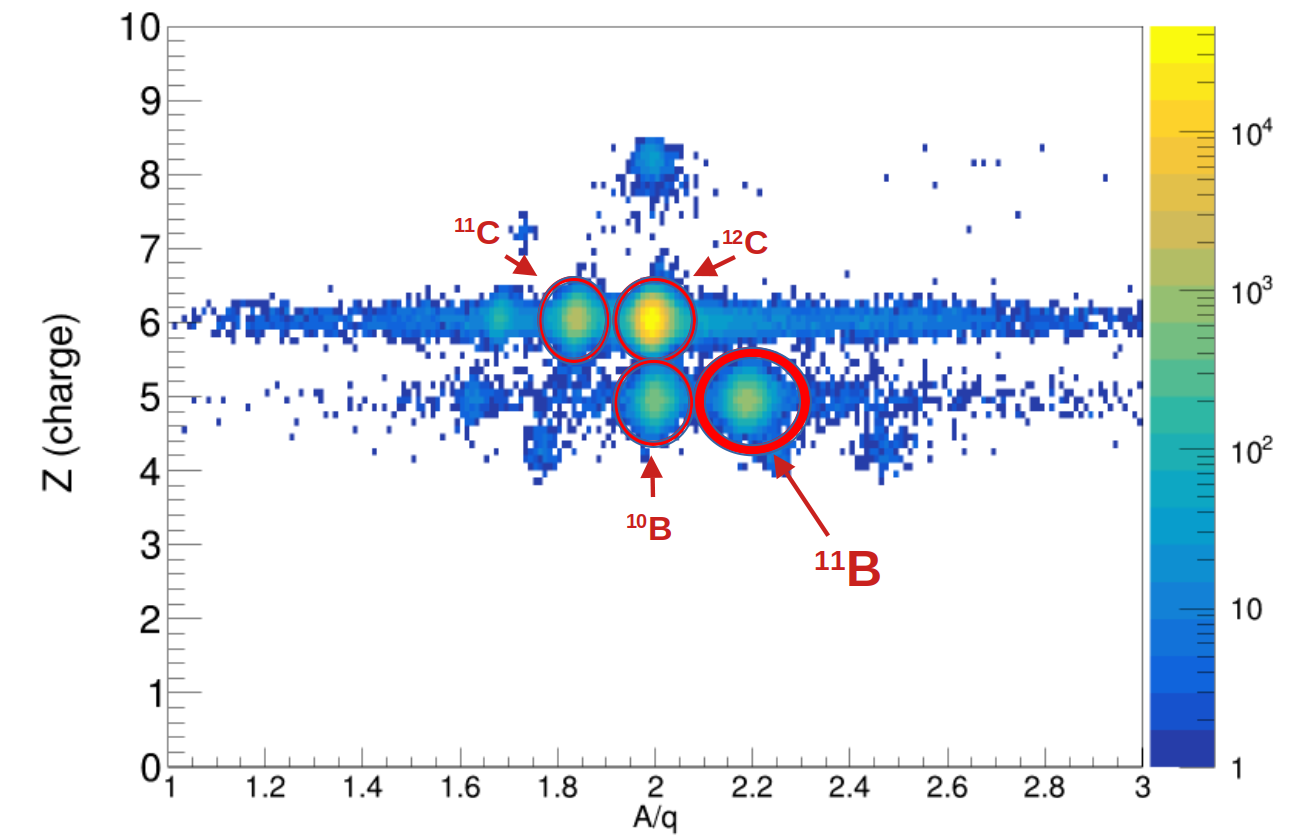
\includegraphics[width=\textwidth,height=12cm,keepaspectratio=true]{Figures/a_over_q_vs_q_plot.png}
    \caption{
	Fragment identification is performed using the correlation between the atomic number $Z$ and the mass-to-charge ratio $\frac{A}{q}$. For the quasi-free scattering (QFS) analysis of the reaction $^{12}C(p,2p)^{11}B$, the fragment of interest is $^{11}B$, which is emphasized with a bold red circle.
    }
    \label{fig:a_q_vs_q}
\end{figure}
For this qualitative analysis, the upper charge bound of $^{11}B$ was determined by locating the intersection point of the Gaussian-fitted distributions corresponding to the $Z=5$ and $Z=6$ peaks. The lower bound was set by applying an offset of minus one unit.\newline
A similar approach was employed to select the specific boron isotope $^{11}B$. The charge selection was performed using the previously defined boundary cuts. To isolate the $^{11}B$ isotopes, the lower bound was determined by identifying the intersection point of the Gaussian-fitted distributions corresponding to the $^{10}B$ and $^{11}B$ peaks. The upper bound was established by measuring the distance from this intersection point to the peak of $^{11}B$.

\subsection{QFS-Protons}
Following the identification of the fragments through precise flight path reconstruction and time measurement, as detailed in the previous subsection, and the subsequent selection of the $^{11}B$ isotope, the analysis focuses on the two correlated protons to fully characterize the quasi-free scattering channel $^{12}C(p,2p)^{11}B$.\newline
For a proper interpretation of the data, it is essential to consider the geometric acceptance of CALIFA during the S444 experiment in 2020. The central \textit{BARREL} region (Ring 3 and Ring 4), covering the polar angular range from $43^{\circ}$ to $88^{\circ}$, was fully operational. In contrast, the forward region, referred to as \textit{iPhos} ($19^{\circ}$ to $43^{\circ}$), was only partially equipped, with a coverage of approximately $35\%$. The forward endcap, known as \textit{CEPA}, was not installed, and the backward barrel remained unoccupied. The corresponding geometry is illustrated in figure \ref{fig:qfs_reac_and_geo}.\newline
\begin{figure}[htpb]
    \centering
    \subfloat[\centering Quasi-free scattering channel $^{12}C(p,2p)^{11}B$]{{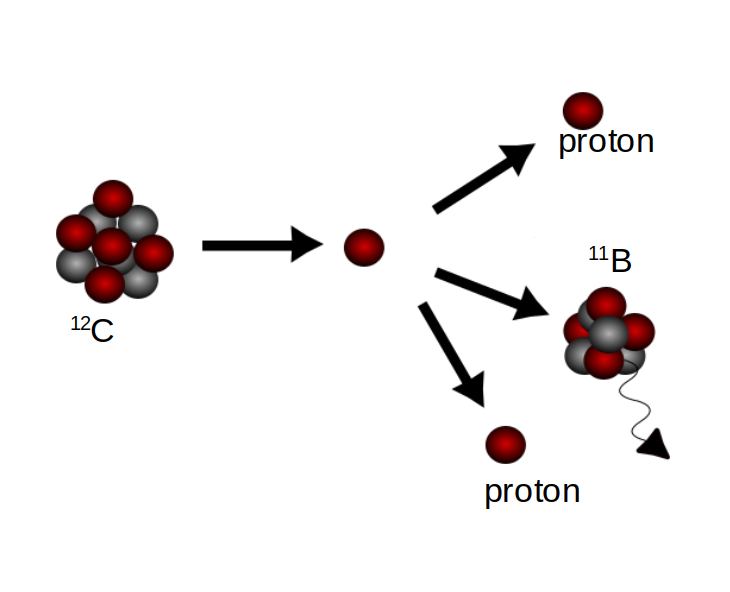
\includegraphics[width=6cm]{Figures/reaction_qfs_model.png} }}%
    \qquad
    \subfloat[\centering Simulated front view of the CALIFA calorimeter in 2020.]{{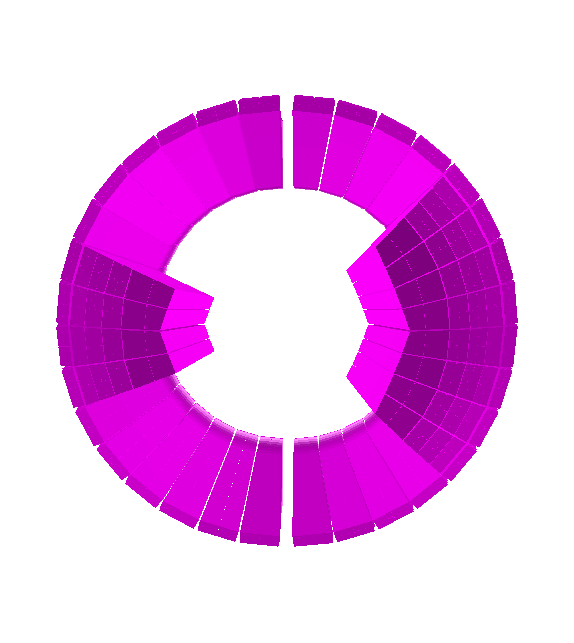
\includegraphics[width=6cm]{Figures/CALIFA2020Front.png} }}%
    \caption{Tagging the $^{12}C(p,2p)^{11}B$ channel with only partly filled CALIFA calorimeter for the detection of the two correlated protons.}%
    \label{fig:qfs_reac_and_geo}%
\end{figure}
For the proton selection and the application of reasonable cuts it is important to understand the processing steps of the raw \textit{mapped} level data to the \textit{cal} level and finally \textit{hit} level data. The \textit{mapped} level data has following structure for each CALIFA hit:
For an accurate proton selection and the application of appropriate cuts, it is crucial to understand the data processing steps from the raw \textit{mapped}-level to the \textit{cal}-level and finally to the \textit{hit}-level. The \textit{mapped}-level data for each CALIFA hit is structured as follows:
\begin{itemize}
\item[$\blacksquare$] CrystalID
\item[$\blacksquare$] Uncalibrated Energy
\item[$\blacksquare$] Slow Component $N_s$
\item[$\blacksquare$] Fast Component $N_f$
\item[$\blacksquare$] WRTS
\item[$\blacksquare$] Time over Threshold
\end{itemize}

The \textit{cal}-level data is structured as in the \textit{mapped}-level, however with calibrated energy by applying the calibration parameters from calibration run to each crystal channel.\newline
For the calibration runs a $^{22}Na$ (with peaks at $511keV$ and $1275keV$) or a $^{60}Co$ (with peaks at $1173keV$ and $1332keV$) is used. For each crystal channel a linear fit on the two photopeaks is performed. Using this fitting function, the uncalibrated energy, expressed in energy channels, can be converted into calibrated energy values.\newline
For the final \textit{hit}-level data the energy-calibrated hits from \textit{cal}-level are merged to clusters.


\footnote{For this analyis, when going from \textit{mapped} to \textit{cal}-level an energy threshold $E_{thr}$ of $100keV$ was applied. All hits with $E_{hit} < E_{thr}$ were omitted in the } 

->Explain cuts that are made in CALIFA and how the clustering works
Plots I need:

%\begin{wrapfigure}{l}{0.25\textwidth}
%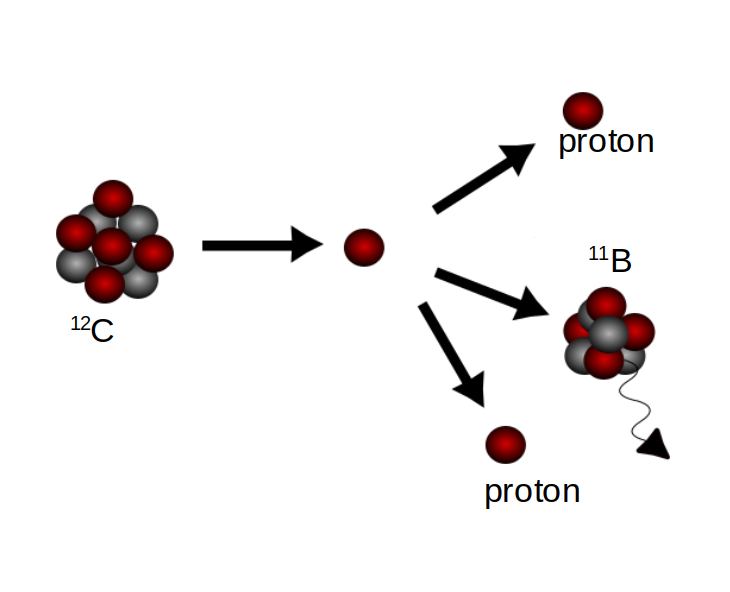
\includegraphics[width=0.9\linewidth]{Figures/reaction_qfs_model.png} 
%\caption{QFS-reaction overview $^{12}C(p,2p)^{11}B$. }
%\label{fig:wrapfig}
%\end{wrapfigure}
->Polar angle correlation plot, explain wixhausen/messel side, this was due to configuration
->Azimuthal angle correlation plot, explain also how this was done
->Opening angle, also with formula, maybe also with simulation? Easy to be done..
->Reconstruction of the inner momentum, make a fit and compare to separation energy, tell that this depends on exact target position and vertex reco point to discussion of separation energy.
->Maybe also correlations between fragment and proton pair, see Chulkov.


\subsubsection{Proton Separation Energy $S_p$}
The proton separation energy $S_p$ of $^{12}C$ from the reaction channel $^{12}C(p,2p)^{11}B$ is defined by the masses and energies of the initial and final state particles in the $^{12}C$ rest frame. One can write the full energy conservation in the rest frame of $^{12}C$:
\begin{equation}
M_{^{12}C} + \gamma \cdot m_p = E_1^* + E_2^* + (M_{^{11}B} + E_{ex})  + T_{^{11}B^*}
\end{equation}
where $E_1^*$ and $E_2^*$ are total energies of the two protons in the $^{12}C$ rest frame, $E_{ex}$ is residual excitation in $^{11}B$ and $T_{^{11}B^*}$ the kinetic energy of the $^{11}B$ in the $^{12}C$ rest frame.\newline
Using this equation, one can express the total binding energy $B$ of the knocked out nucleon:
\begin{equation}
B = S_p - E_{ex} = M_{^{12}C} - M_{^{11}B} - E_{ex} - m_p = E_1^* + E_2^* + T_{^{11}B^*} - \gamma \cdot m_p - m_p
\end{equation}
Using Lorentz transformation from lab to 12C rest frame one can obtain for $E_1^*/E_2^*$:
\begin{align*}
E_{1/2}^* &=  \gamma \cdot m_p + \gamma \cdot T_{1/2} - \beta \cdot \gamma \cdot p_{1/2} \cdot cos(\theta_{1/2})
\end{align*}
The kinetic energy of the $^{11}B$ in the $^{12}C$ rest frame can be written as:
\begin{align*}
T_{^{11}B^*} &= \frac{p_i^2}{2 \cdot M_{^{11}B}}
\end{align*}
with $p_i$ the inner momentum of the proton knocked out of the $^{12}C$ projectile, see equation \ref{eq:miss_mom}.
Putting this in the previous equation one finally gets for the binding energy $B$:
\begin{equation}
B = (\gamma - 1)\cdot m_p + \gamma \cdot (T_1+T_2) - \beta \cdot \gamma \cdot(p_1*cos(\theta_1) + p_2*cos(\theta_2)) + T_{^{11}B}
\end{equation}\label{eq:sep_energy}
For $E_{ex} = 0$, i.e. the fragment $^{11}B$ in the ground state, the binding energy $B$ is equal to the one proton separation energy $S_p$\footnote{Since the $^{11}B$ fragment predominantly remains in its ground state---implying that, in most cases, the outermost protons are removed---the binding energy $B$ and the proton separation energy $S_p$ are used interchangeably, also due to the limited energy resolution.}. \newline
As for the S444 experiment no target detector tracking system was available. Consequently the energies as well as the azimutal ($\phi$) and polar($\theta$) angles of the two correlated protons had to be fully reconstructed using the CALIFA calorimeter. The calorimeter provided an energy resolution $\frac{\Delta E}{E}(@100MeV) \lesssim 1 \%$, along with angular resolutions of approximately  $\Delta \phi \approx \frac{6}{\sqrt{12}}^{\circ}$, and $\Delta \theta \approx \frac{2}{\sqrt{12}}^{\circ}$.
The best way to visualize the separation energy $S_p$ id to plot it against the summed energy of the two protons in the $^{12}C$ rest frame as shown in figure \ref{fig:sep_energy}. Two vertical lines are visible. They correspond to the two QFS-reaction types within the $CH_2$ target: the proton within the $^{12}C$ projectile can either scatter on the hydrogen (proton-like) part of on the carbon part of the plastic target. For the first case only the separation energy $S_p$ as derived in equation \ref{eq:sep_energy} is necessary to remove the proton of the projectile within the $^{12}C$ nucleus. In the second case the QFS-reaction is between two protons both bound within a carbon nucleus -- the projectile carbon and the target carbon part. Herefore more energy is needed to free both protons from their nuclear bond. This corresponds to the left vertical line in figure \ref{fig:sep_energy}. It should be noted that the reconstructed one-proton separation energy $S_p$ is shifted with respect to the mean value of $\approx 16 MeV$. For a precise measurement the accurate position of the target and the reaction vertex would be needed, as well as a precise measurement of the kinetic energy of the incoming $^{12}C$ would be required (for the actual measurements the beam energy value was set to $400 AMeV$). 
\begin{figure}[htpb]
    \centering
    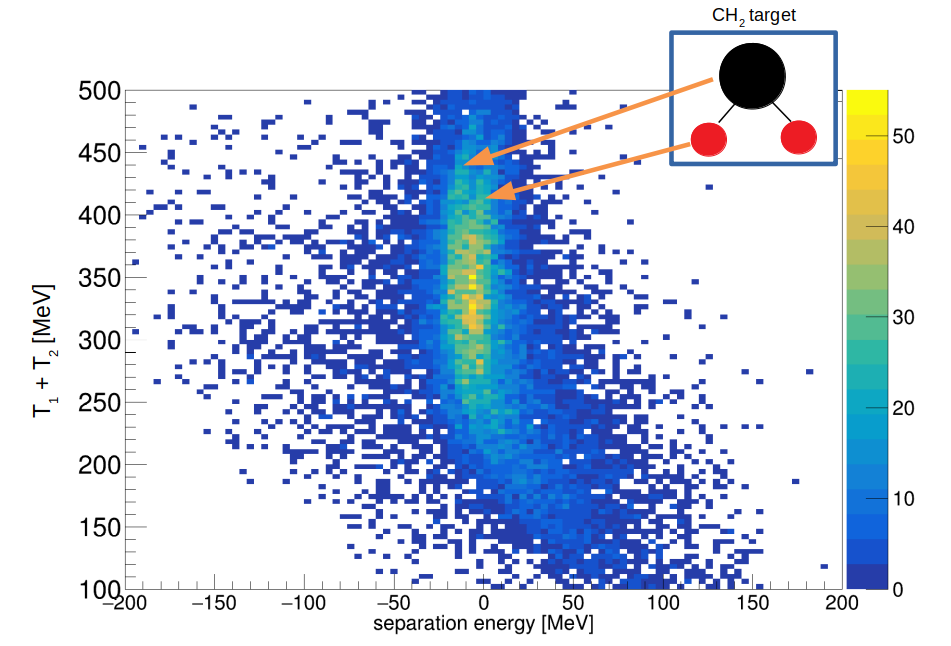
\includegraphics[width=\textwidth,height=10cm,keepaspectratio=true]{Figures/sep_energy_vs_sum_energy.png}
    \caption{
	Sum of the kinetic energies of the two correlated protons ($T_1/T_2$) versus the one proton separation energy $S_p$. Since this energy is needed to solve the proton from the nucleus' core, it's valuehas conventionally a negative sign.  	 
    }
    \label{fig:sep_energy}
\end{figure}

\subsection{Reconstruction of excited$ ^{11}$B states}
->Show level scheme of 11B, explain excited states and why it is not expected to see any peaks at 4.4 MeV.
->Explain Doppler correction (this is really the key point of the CALIFA, why it is highly segmented)
-> show all conditions that you apply
-> This comm. exp. has shown that we can really pin down reaction mechanism and we are ready for exciting p2p experiments
-> Limitations: CALIFA was only partly filled for this exp. 
\subsection{Fission via Quasi-Free Scattering reaction}
-> shortly explain the challenges behind, idea should be in the theory part. Also mention that this was complementary experiment to Coulex Exp, where nature paper was submitted
-> mention that TUM Munich group was strongly involved
-> Charge reconstruction is done, mention the papers and publications
-> One really interesting aspect would have been to pick out specific reaction channels, eg. with one fission fragment being a thin isotope and look at the gamma spectrum. 
-> the issue there is of course that precise thin isotope cannot be selected yet. But from CALIFA side this was motivation to improve the clustering algorithm, especially for fission reactions, where you have lot more hits in CALIFA. And there especially looking at low energy hits from gammas, which can be quite sparse.
-> This should then be the introduction for the next section about clustering.
